\documentclass{hissymp}
\usepackage[dvipdfmx]{graphicx}
  \usepackage[utf8]{inputenc}
  \usepackage[T1]{fontenc}
  
\usepackage[utf8]{inputenc}
\usepackage[T1]{fontenc}
\usepackage{graphicx}
\usepackage{grffile}
\usepackage{longtable}
\usepackage{wrapfig}
\usepackage{rotating}
\usepackage[normalem]{ulem}
\usepackage{amsmath}
\usepackage{textcomp}
\usepackage{amssymb}
\usepackage{capt-of}
\usepackage{hyperref}
\author{\texttt{S}}
\date{}
\title{}
\hypersetup{
 pdfauthor={\texttt{S}},
 pdftitle={},
 pdfkeywords={},
 pdfsubject={},
 pdfcreator={Emacs 26.1 (Org mode 9.1.9)}, 
 pdflang={Jp}}
\begin{document}


\begin{abstract}
\label{sec:orgcf61c69}
At graduate research, 
although the process is more important than the results,
most students don't notice it.
Because the guild system is nice to learn the process,
the graduate reseach possesses a kind of
relationship between 
a mentor and a padawan learner.

On this project, 
we are developing a system for
noticing importance of learning process,
ornb, whose specifications and 
the connections to a static web system, jekyll,

\end{abstract}

\begin{keyword}
keyword 1, keyword 2, keyword 3, keyword 4, keyword 5
\end{keyword}

\maketitle
\section{Introduction}

\label{sec:org62c9579}
\subsection{背景I - 大学の学び}
\label{sec:orgbf163a9}
今日の大学教育は,フンボルト理念を基礎としている.その通説を
\begin{quote}
近代大学の出発点は1810年に創設されたベルリン大学である。この大学の基本構想を作ったのは、ヴィルヘルム・フォン・フンボルトであり、近代大学はこのフンボルト理念から始まった。フンボルト理念の中核は研究中心主義にある。つまり、大学は教育の場である以上に研究の場であるという考え方は、このフンボルトから始まった。これがドイツばかりでなく、世界の大学を変えた。
\end{quote}
と潮木はまとめている.
\begin{itemize}
\item アルカディア学報(教育学術新聞掲載コラム),No.246
\end{itemize}
この後,潮木はその著書でフンボルト理念が単なる「神話だった」と力説している.

日本の工学を中心とする学部においては,
研究至上主義としてのフンボルト理念が,
大規模講義形式の授業への出席,
レポートや期末試験を経て単位を取得する仕組みに繋がっている.

しかし,学生は,意欲的に授業に参加し,
自らが参加者となり授業に出席することで,
知識を得ようとする姿勢が見受けられない.
「単位さえあればいい」あるいは「卒業して就職さえできればいい」という
本音と,「眠い」という実感によって,
大学で授かるべき知識について魅力を感じなくなっている.
あるいは社会に出て,すぐに実用できるスキル
実用できるスキルの習得,例えば,英会話や論文作成術を
身につけようとする.

したがって,授業の内容の重要性に気づくことなく,
レポートや期末試験の前にレジュメを確認しその内容を提出する.
つまり,内容や過程を重要視せず,結果のみを重要としている.

つまり,現在学生の知識習得に役立つと思って課されている
レポートや試験は,
結果のみを求めているという誤ったメッセージとして,
学生が受け取っている可能性がある.

\subsection{背景II - 大学生は徒弟制を否定しがち}
\label{sec:org4ae3b3e}
ところが,
最新の教育を行うと看板を掲げている大学に通う今日の学生は,
大学は研究の場であるという認識が薄く,
卒業研究や,研究室におけるゼミへの参加に
どのようなスタンスで取り組めがいいか
明確には理解できない.
ある意味,学生には,研究室とは,
「大学システムが切り捨てようとして来た,徒弟制的な制度である」
ということは全く脳裏にない.
\begin{quote}
1989年にグロスハンスの指摘によれば,
西ヨーロッパとほかでもない米国において

中略

徒弟制は最も価値のある,
しかも最も力のない労働者を統制するための伝統的な形態だと長い間みなされていた.
LaveWenger[p.41]
\end{quote}
これが,徒弟制に対する一般的な意識であり,大学生の多くもそのように認識していると考えられる.

\subsection{目的}
\label{sec:org9f8bdbb}
次節で示す通り,このような旧態然とした徒弟制も現代的な視点で
見直しが進められている.
本プロジェクトで提供しようとするシステムは,
\begin{itemize}
\item 研究室は徒弟制
\item 学生はそれを知らない
\end{itemize}
という前提のもとで,徒弟制を新たな学習形態として提供することを
目的としている.

次節では,どのような経緯で徒弟制が見直されて来たか,また,
学習がAM/PMという視点によってどのように捉えられているかを
明らかにする.
その上で,近代的な徒弟制を研究室活動に導入するのに
必要となる仕様を列挙し,それに基づいた実装デザインを示す.

\section{徒弟制の見直し}
\label{sec:org3ddde17}
\subsection{状況に埋め込まれた学習}
\label{sec:org090ba02}
1991年にレイヴとウェンガーによって,
  「状況に埋め込まれた学習」あるいは「正統的周辺参加」
  という学習形態・概念が提案された.
  彼らは,アフリカの仕立て職人や助産婦の育成法を社会学的に詳しく調査した結果,
  徒弟制のなかに学びの本質があると指摘した.
少し複雑ではあるが,その概念をもっとも短くまとめたと思われる箇所を以下にそのまま書き写す.
\begin{quote}
学習はいわば参加という枠組で生じる過程であり,
個人の頭の中でではないのである.
このことは,とりもなおさず,
共同参加者の間での異なった見え方の違いによって学習が媒介されるということである.
この定義では「学ぶ」のは共同体である,
あるいは少なくとも,
学習の流れ(context)に参加している人たち,といえよう.
学習はいわば,共同参加者間にわかち持たれているのであり,
一人の人間の行為ではない.
生産過程では徒弟(見習い)が益々増大していく
参加によってきわめてドラマティックに変容していくものではあるが,
この変容の発生の場と発生の条件は,さらに広範囲の過程そのものである.
徒弟の親方たち自身が共同学習者としてふるまうことを通しどれほど変化するか,
したがって,習熟されている技能でもその過程でどれほど変化するか.
実践者の共同体がより大きくなると,
徒弟の形成によって共同体は自らを再生させるが,
同時に変容もすると考えられる.
LaveWenger[pp.8-9]

中略

また新参者を親方,ボス,あるいは管理者と深く対立する関係に陥らせる,参加させるよりも非自発的に隷従させるなど,これらの条件は実践における学習の可能性を部分的に,もしくは完全に,歪めてしまうと唱えた.
 LaveWenger[p.42]
\end{quote}
と記している.

\subsection{AM/PM}
\label{sec:org47bba06}
1998年数学者のSfardは,Lave and Wengerの考えを受け,
学習者,教授者,研究者のあり方について
AM(Acquisition Metaphor)とPM(Participation Metaphor)と名付けた.
学習に対する従来の考え方であるAMは,個人が知識を習得することを目標とし,
「学習」とは何かを獲得することであった.また,「知る」は個人が所有するものであると
していた.一方で学習に対する新しい考えであるPMは,学習の目標は共同体の構築であり,「学習」とは参加者となることである.学習者は,徒弟であり,教授者は,有識の参加者と定義した.
つまり,個人ではなく,教授者,学習者がチームとして,また徒弟制を築くことでお互いお互いの知識構築が捗る仕組みとなっている.

表\ref{tab:org00bb5a5}

\begin{table*}[bt]
\caption{\label{tab:org00bb5a5}
Acquisition metaphorとParticipation metaphorの比較.}
\centering
\begin{tabular}{lll}
\hline
Acquisition metaphor & 要素 & Participation metaphor\\
\hline
個人を豊かにする & 学習の目標 & 共同体の構築\\
何かを獲得する & 学習するとは & 参加者となる\\
受容者,再構築者 & 学習者 & 周辺参加者,徒弟\\
供給者,促進者,仲裁人 & 教授者 & 有識の参加者\\
資産,所有物,一般商品 & 知識,コンセプト & 実践,論考,活動の一側面\\
持つ,所有する & 知るとは & 所属する,参加する,コミュニケーションをとる\\
\hline
\end{tabular}
\end{table*}

\subsection{PMの実践例と学生の受け止め方}
\label{sec:org7caf9df}
関西学院大学理工学部・情報科学科で西谷が参加型学習を実践している
数式処理演習,モデリング物理学という授業がある.
一般的なアクティブラーニングと違い,
これらの授業では,学生同士が自主的にペアを組み
授業中課題や期末試験をペアあるいはチームで受け,
彼らの点数は全く同じとなるようにつけられる.

数式処理演習では,数式処理ソフトMapleまたはPythonを用いて,
センター試験,微積分,線形代数の基礎的な問題を解くスキルを身につける.
また,課題やテスト結果の評価は,ペアで共通するものとしている.
ここで重要なのは,問題を解くスキルを身につけるはもちろんであるが,ペアで課題に取り組むことである.
二人一組のチームを生成することで,「相方の足を引っ張らないように」という思考に至り,互いが怠けることなく,授業や課題に意欲的に取り組む.
その結果,互いに高め合い,知識の定着につながる.
「共同体の構築」,「参加する」これがPMという考え方である.
しかし,中には知識の定着に至らない学生もいる.
\subsubsection{客観的な事実を記述}
\label{sec:org3c29a79}
\begin{itemize}
\item 一つ目の要因はペアによる演習のため,
一人が作業すれば課題をクリアできる点である.
つまり,問題毎に役割を振り分け 
片方が問題を解いている時,
もう片方は携帯を見るなど考える事を
完全にやめることがある.
一緒に考えることをせず,
「休憩」の時間を作ることで
知識定着を目的とするのではなく,
課題達成,単位習得の事のみを考えた結果である.

\item 二つ目は,ペアで課題を一つ提出することが,
いわゆる出席点となるため
一人が授業を欠席しても,
点数が減点されることがない点である.
これは,一つ目に述べた要因より酷い例であり,
日にち毎に出席する担当を決めることで
授業に出席,参加すらしない場合があった.
\end{itemize}

結果的に見るとこの授業は,
PMといった考え方を気づかせる授業ではなく
学生にとって,「授業に出なくても良い楽に単位を取れる授業」
という風に見受けられた.

また,個人での学習よりも互いに高め合い,知識・スキルを
習得するといったペアは一部であり,
PMを理解した生徒,優秀である生徒と
そうでない生徒がペアを組んだ場合,
前者がほとんどの課題をこなし,
後者はほとんど考えないというパターンも存在した.

参加型学習の実践の失敗
何が悪いかを分析


\section{卒論・ゼミ}
\label{sec:orgd234283}

客観的な事実の記述
\begin{itemize}
\item 西谷研究室では,生徒の出席率が悪い.
これの要因は,他人任せであることが一番大きい.
「誰かが出席していれば,なんとかしてくれる」,
「欠席による出席者より理解が遅れるという危機感の無さ」,
「プライベートとゼミとの優先順位がおかしい」
等が挙げられる.
\end{itemize}



卒業研究やゼミにおいても,教授や先輩が後輩に計算機の使い方や,
プログラミング,レポートの書き方を教える.
この時,後輩は自らの意思で参加するという考え方であるべきだ.
西谷研究室では,後輩が参加者となり先輩から学ぶという風潮が見受けられない.
後輩は,卒業研究を発表すること,
結果のみを考えており,卒業研究を発表するまでの過程の重要性に気づいていない.

\section{構築システムのアイデア}
\label{sec:org13d3b00}
\subsection{新しい徒弟制と古い徒弟制,西谷研でどうするよ?}
\label{sec:orge480f70}
\begin{itemize}
\item このような参加型の学習を西谷研で実践するのに何が必要か?
\item 徒弟制の本質
\item 親方と徒弟の関係
\begin{itemize}
\item 古いよね
\item 見習い?
\item 習慣
\end{itemize}
\item 先輩の仕事
\item 硬い上下関係ではなく,参加して学ぶ
\item 徒弟のモチベーション,参加意欲
\item 教える方も,確固とした知識として身につけることができる
\item 今まで何で,教えなかった
\item ダンスはあるけど,
\item 後輩と勉強する機会がない
\item そういう機会がないから
\item 優先順位がおかしい
\item 共同体への参加というのを気づいていなかった.
\item 同じやろ
\item 声かけ
\item 目に見える形にして共有する
\end{itemize}

学べる人はどこでも学べる?

\subsection{[o] 日報}
\label{sec:orge7ba4c8}
\begin{itemize}
\item 自分がやったことの記録
\item blogはそのつもり
\item 見た目って大事
\item 手軽にできる
\item org
\item my\_help
\end{itemize}

\subsection{[x] 罰を与える? }
\label{sec:orgac3ea1b}
\begin{itemize}
\item 卒業はなし
\item 恥ずかしい
\item 何をするとしでかしたと思う?
\item 名指しで言われる
\item 全体の目が通るところで糾弾
\item てのはめんどいんで,スタンプ集めに変更
\item 糾弾せよ!!!自己批判せよ!!!
\end{itemize}
\subsection{[o] ペアプロ}
\label{sec:org29b49db}
\begin{itemize}
\item ゼミ? テキスト?
\item 徒弟制と大学,スキルと記述的記憶の違い
\item スキルの伝達をチェックする?
\item free riderが増える
\item コピペはダメ!
\item ペアでの作業
\item ペア評価
\item 責任,サボれない
\end{itemize}

\begin{quote}
ただ始めること.これがたぶん生産性の鍵なのだ.
ペアプロが機能する理由は,「相方とペアプロ作業を予定する」ことで,
「作業を始めることをお互いが強制する」からに違いない
(原文より訳出).
Joel Spolsky 著,青木靖訳「Joel on software」(オーム社,2005)p.133.
\end{quote}

\begin{itemize}
\item チェックにならない.
\item だから,skypeとかが必要.

\item scheduling
\item 予定の強制,スタンプ集め
\end{itemize}
\subsection{[o] スタンプ集め}
\label{sec:org3742486}
例えば
\begin{itemize}
\item 全員jekyllを入れて,blogを晒す
\end{itemize}
というゼミで実行した課題があるとする.そいつを全員が実行したかどうかを,教えた方がチェックする.
手順は以下の通り,
\begin{itemize}
\item 欠席者が出席者に聞く
\item 出席者がスタンプを押す
\item それが埋まってなかったら卒業なし.
\end{itemize}
これを自動化するシステム.

いっぺん聞いたら他の人に教えるのはあり.
そうすると,教えることによる記憶強化の可能性が高まる.
また,不明瞭な点のあぶり出しが可能になる.

\subsection{[ ] チームによる課題達成}
\label{sec:orgf929b20}
\begin{itemize}
\item こいつをシステムにする?
\item こいつを徒弟制にする?
\item こいつをPMの実践に昇華する
\end{itemize}
\subsection{[ ] 卒業研究や授業の課題において,その過程が重要である.}
\label{sec:orgcc1312b}
自ら行った事を過程も含めてレポートとしてまとめ,公開することで,知識構築に繋がると考える.
レポートにまとめることは,それらの過程も含めて理解する必要がある.また,自らの復習となり,より知識として身につく.
次に,公に公開することで,日本語や文の構築に気を使うため,学んだことの理解だけでなく,レポート作成の知識も身につくといった利点がある.
また,公開することで他の人から指摘や意見をもらうことができるため,そこで議論を広げることで,
より知識が定着する.
これらを実現するために,org-mode,ruby,my\_help,jekyll,GitHub Pagesを用いて過程の重要性を気づかせるシステムを提案する.

\subsection{[ ] スイッチ}
\label{sec:org24bb85e}
\begin{itemize}
\item 象(感情)と象使い(理性)
\item サボっているように見えて,実は混乱している
\item 双曲性の話
\item 縛る
\item defaultを変える
\end{itemize}

\subsection{[o] org-mode = 便利なmark down}
\label{sec:org8c394b8}
org-modeは,Emacs上で動作するアウトライナーであり
プレーンテキストの文書作成環境である.
ノートの保存,TODOリストの管理,スケジュールや時間の管理,
また発表原稿やスライドの作成など様々な用途に対応している.
また,コードの実行はもちろん,リンク付け,テーブル表記の入力,
図や表の表示,ライブ計算,HTMLや\LaTeX{}への変換等の
機能も兼ね備えている.
今回のレポートとなる文書の作成するために,org-modeを用いる.

\subsection{[o] my\_help == 直交補空間}
\label{sec:orge0e66ec}
ファイル構造において,メモやレポートが増えれば増えるほどchunkingする.
chunkingすることにより,構造が深くなる.その結果,レポートやメモの場所
が把握できなくる.
my\_helpは,直交補空間を実現した知識構築を補助するツールである.
ディレクトリに拘束される事なく,メモやレポートを作成できる利点があるため,
どこからでもアクセスできる.

directoryってのは知識のマップ.
知識が大きくなると,chunkingする.
深くなる.
迷子になる.
my\_helpってのは直交補空間に置かれている.
いつでもaccessできて便利.

\subsection{[x] repl == jupyter notebook}
\label{sec:org650416d}
てのは試行錯誤.
loopがある.
jekyllとか,github, と結びつけて,システムにならないか?

\subsection{[o] jekyll == 晒すと何がいい?}
\label{sec:org59dc7f7}
jekyllはRubygemsで提供されている静的サイトジェネレーターである.
テーマや構成を変更することができ,好みのサイトを作成できる.
今回の文書の公開をjekyllで行う.
\begin{itemize}
\item 文章,文を気にする,
\item 共有しやすい,
\item 形になる,
\begin{itemize}
\item report
\item 他人事だと思っているから
\item 自分が学んでいることとの関連性を自覚する
\item 深く理解する
\item 経験知識に変える,説明する,議論する
\begin{itemize}
\item 徒弟制ではない,大学システム
手に職を,中世のシステム
\end{itemize}
\end{itemize}
\end{itemize}

\section{ornbの仕様}
\label{sec:org7220395}
\subsection{スタンプ集め}
\label{sec:org63e8492}
例えば
\begin{itemize}
\item 全員jekyllを入れて,blogを晒す
\end{itemize}
というゼミで実行した課題があるとする.そいつを全員が実行したかどうかを,教えた方がチェックする.
手順は以下の通り,
\begin{itemize}
\item 欠席者が出席者に聞く
\item 出席者がスタンプを押す
\item それが埋まってなかったら卒業なし.
\end{itemize}
これを自動化するシステム.

いっぺん聞いたら他の人に教えるのはあり.
そうすると,教えることによる記憶強化の可能性が高まる.
また,不明瞭な点のあぶり出しが可能になる.

\subsection{レポートの作成と公開}
\label{sec:org782498e}
まずはじめにレポート作成から公開までの流れは図\ref{fig:org563b34f}のようになる.
\begin{figure}[htbp]
\centering
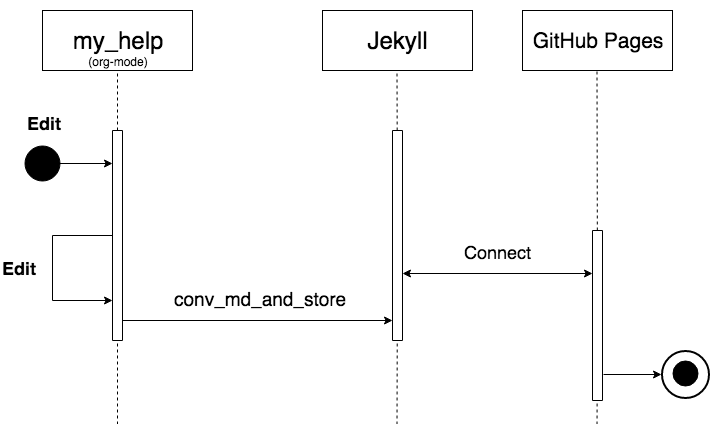
\includegraphics[width=8cm]{./images/myhelp_to_jekyll.png}
\caption{\label{fig:org563b34f}
レポート作成から公開までの流れ}
\end{figure}


次に,レポートの作成について述べる.
レポートの作成はRubygemseで提供されている,
my\_helpを用いる.

my\_helpを以下の方法でインストールする.
\begin{quote}
\begin{verbatim}
gem install my_help
\end{verbatim}
\end{quote}

次に,my\_helpにblogというlistを作成するために,
以下のコマンドを実行する.

\begin{quote}
\begin{verbatim}
my_help new blog
\end{verbatim}
\end{quote}

これで新しいlistが作成される.
次にblogの内容を編集するため,以下を実行する.
\begin{quote}
\begin{verbatim}
my_help edit blog
\end{verbatim}
\end{quote}

編集画面では,タイトルをつけた後,タイトルの横に
図\ref{fig:org2659c98}のような日付を付けることとする.
\begin{figure}[htbp]
\centering
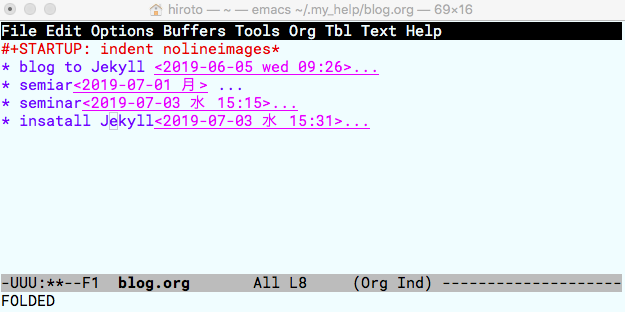
\includegraphics[width=13cm]{./images/add_date.png}
\caption{\label{fig:org2659c98}
日付を付ける例}
\end{figure}

また,以下のコマンドで日付を付ける事が出来る.
\begin{quote}
\begin{verbatim}
Control-u Control-c .
\end{verbatim}
\end{quote}

あとは,Blogの内容を書き込んでいく.

\subsection{Jekyllのインストールと実行}
\label{sec:org4d2ad32}
Blogの作成と公開はJekyllとGithub Pagesを用いる.
以下にその手順を記述する.
\href{https://qiita.com/daddygongon/items/9b7182db29861744fc79}{jekyllのinstallとGitHub Pagesとの連携}

はじめに,Jekyllをインストールする.
\begin{quote}
\begin{verbatim}
gem install bundler jekyll
\end{verbatim}
\end{quote}

次にローカルサーバを立ち上げる.
\begin{quote}
\begin{verbatim}
jekyll new my-awesome-site
cd my-awesome-site
bundle exec jekyll serve
\end{verbatim}
\end{quote}
\end{document}
